\documentclass[11pt]{article}
\usepackage[utf8]{inputenc}

\usepackage{geometry}
\geometry{a4paper}

\usepackage{graphicx}
\usepackage{hyperref}
\usepackage[parfill]{parskip}
\usepackage{amsmath, amssymb}
\usepackage{fdsymbol}
\usepackage{color,soul}

% remove section numbering
\makeatletter
\renewcommand{\@seccntformat}[1]{}
\makeatother

% make subsubsection italic
\usepackage{sectsty}
\subsubsectionfont{\itshape}

\renewcommand{\arraystretch}{1.4}

\title{Probability Theory \& Statistics}
\date{}
\author{}

\begin{document}
\maketitle
\clearpage

\section{Nonlinear Regression}

\subsection{Curve Fitting}

Consider a set of \(m\) data points, \((x_{1},y_{1})\), \((x_{2},y_{2})\)
\ldots, \((x_{m},y_{m})\) and a model function
\begin{align}
\widehat{y} = f\left( x,\boldsymbol{\beta} \right),
\end{align}
that depends on an independent variable \(x\) and a set of \(n\) parameters, 
\(\boldsymbol{\beta} = (\beta_{1},\beta_{2},\ldots,\beta_{n})\),
with \(m \geq n\), 
where \(\boldsymbol{\beta}\) is a \emph{vector} of parameters. 
The hat notation \(\widehat{\cdot}\) denotes that \(\widehat{y}\) is an \emph{estimate of \(y\)}. 

\emph{Curve fitting} corresponds to finding a vector of parameters 
that best fits the curve given the data,
i.e., \(\widehat{y}\) is a best estimate of \(y\).

A common measure of best fit is in the \emph{least-squares} sense, 
where the sum of squared residuals
\begin{align}
S = \sum_{i = 1}^{m}r_{i}^{2}
\end{align}
is minimized, given the residuals (the \emph{in-sample prediction errors})
\begin{align}
r_{i} = y_{i} - f(x_{i},\boldsymbol{\beta})
\end{align}
for \(i = 1,2,\ldots,m\).

The minimum value of \(S\) occurs when the gradient is zero. 
(See the example below for a numerical example). 
Since the model contains \(n\) parameters there are \(n\) gradient equations:%
\footnote{Can you derive this equation?}
\begin{align}
\frac{\partial S}{\partial\beta_{j}} = 
2\sum_{i}^{}r_{i}\frac{\partial r_{i}}{\partial\beta_{j}} = 0,\qquad (j = 1,2,\ldots,n).
\end{align}
In a nonlinear system, 
the derivatives \(\partial r_{i}/\partial\beta_{j}\) are functions of both the
independent variable \emph{and} the parameters, 
so don't typically have closed-form solutions.%
\footnote{Why?} 
Instead, numerical methods must be
employed with initial values provided for the parameters.

The parameters are iteratively refined by successive approximations.
\begin{align}
\beta_{j} \approx \beta_{j}^{k + 1} = \beta_{j}^{k} + \Delta\beta_{j}
\end{align}
where \(k\) is the \(k\)th successive iteration. 
The problem can be reformulated as a system of \(n\) simultaneous linear equations that
form the basis for a Gauss-Newton solver for nonlinear least squares problems.

\subsection{Convergence Criteria}

The iterative method isn't guaranteed to find a minimum, 
nor is it guaranteed to even decrease from one iteration to the next. 
One possible criterion for convergence is,
\begin{align}
\left| \frac{S^{k} - S^{k + 1}}{S^{k}} \right| < a
\end{align}
where \(a\) can be chosen somewhat arbitrarily, 
e.g., setting \(a=0.001\) is a common value. 
Many other criteria exist for stopping the algorithm. 
Because the method isn't always guaranteed to converge, 
a limit is usually set on \(k\).

\subsection{Second-order Polynomial Fitting}

Consider the following dataset consisting of four response datapoints,
\(y_{1}\), \(y_{2}\), \(y_{3}\), \(y_{4}\) measured at four concentrations,
\(x_{1}\), \(x_{2}\), \(x_{3}\), \(x_{4}\), 
in a dose-response experiment.

\begin{table}[h!]
\centering
\begin{tabular}{| l | l | c |}
\hline
$x_{i}$  & $y_{i}$ & $r_{i}$\\\hline
\(1\) & \(6\) & \(6 - \beta_{1}(1)^{2}\) \\
\(2\) & \(5\) & \(5 - \beta_{1}(2)^{2}\) \\
\(3\) & \(7\) & \(7 - \beta_{1}(3)^{2}\) \\
\(4\) & \(10\) & \(10 - \beta_{1}(4)^{2}\) \\\hline
\end{tabular}
\caption{%
Hypothetical measurements from a dose-response experiment.
}
\label{tab:residuals}
\end{table}

The response model function is assumed to be a second-order polynomial
function of the concentration,%
\footnote{Although the independent variables are nonlinear, 
\(f\) is a linear function of the \emph{parameters}, 
corresponding to a linear regression as opposed to a nonlinear regression. 
The example is nonetheless still useful for understanding least-squares methods.}
\begin{align}
y = \beta_{3} + \beta_{2}x + \beta_{1}x^{2}
\end{align}
with \(\beta_{3}\) and \(\beta_{2}\) further set to zero in this
experiment. Table \ref{tab:residuals} calculates the residuals for this model function.
Substituting the residuals into the equation for the sum of squared
residuals gives,
\begin{align}
S\left( \beta_{1} \right) = \left( 6 - \beta_{1} \right)^{2} + \left( 5 - 4\beta_{1} \right)^{2} + \left( 7 - 9\beta_{1} \right)^{2} + \left( 10 - 16\beta_{1} \right)^{2}
\end{align}
that has a single partial derivative,
\begin{align}
\frac{\partial S}{\partial\beta_{1}} = 708\beta_{1} - 498.
\end{align}
Setting the partial derivative to zero and solving yields
\begin{align}
\beta_{1} = \frac{498}{708} = 0.7033898\ldots
\end{align}
giving
\begin{align}\label{eq:ls-fit}
\widehat{y} = 0.703x^{2}
\end{align}
the best model fit in a least-squares sense.

Figure \ref{fig:ls-fit} plots the hypothetical data and the best fit in a least-squares 
sense assuming a quadratic model function. 
In the supporting R code we compare equation \ref{eq:ls-fit} to R's built in (nonlinear) least-squares
numerical optimizer with starting value \(\beta_{1} = 1\).

\begin{figure}[h!]
\centering
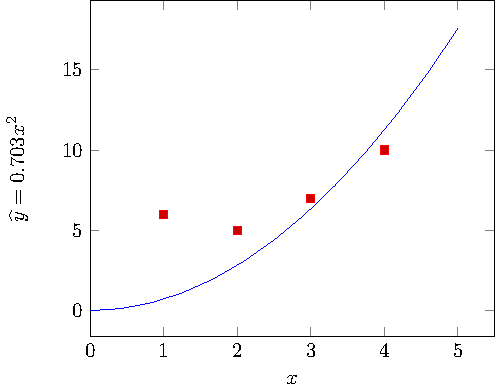
\includegraphics[width=0.5\linewidth]{tikz/figure1}
\caption{%
Plot of example data and computed best fit.
}
\label{fig:ls-fit}
\end{figure}

\subsection{Matrix Notation}

It's often useful to represent fitting and optimization problems as \emph{matrices}. 
In matrix notation, 
the equations without residuals are
\(\boldsymbol{y} = \boldsymbol{X}\beta\) with
\begin{align}
\boldsymbol{y} = [6,5,7,10]^{T},\qquad \boldsymbol{X}=[1,4,9,16]^{T}
\end{align}
where \([\cdot]^{T}\) represents a \emph{matrix transpose} 
and \(\beta = [\beta_{1}]\) is a \emph{scalar}, i.e., just a number.

Solving for \(\beta\) yields the estimate,
\begin{align}
\widehat{\beta} = 
\left( \boldsymbol{X}^{T}\boldsymbol{X} \right)^{- 1}\boldsymbol{X}^{T}\boldsymbol{y} = [ 0.703],
\end{align}
In the supplementary R code we solve this system using R's base matrix operations,
yielding \(\beta = 0.703\) in agreement with the other calculations.

\subsection{Uncertainty}

\subsubsection{Definition}

The problem stated so far has been a \emph{deterministic} algorithm for
minimizing the sum of squared residuals. 
The parameters that optimize
the problem produce a best fit curve in a least-squares sense. 
The \emph{point estimates} calculated in the fitting 
(each change in the independent variable \(x\) results in a single point \(y = 0.703x\) in
the curve fit) don't provide a measure of uncertainty, i.e., there is a
single curve, and we are completely confident that it is the best curve.

But are we really completely certain the ``best fit'' really is the best fit? 
Instead of a point estimate, 
it would be useful if could instead provide an interval of fit, 
with a probability associated to that interval, 
conditional on the value of the independent variable \(x\).

Symbolically we write this as,
\begin{align}
P\left( a \leq Y(X) \leq b\ |\ X = x\right) \in [0,1]
\end{align}
where the \emph{response}, \(Y=y+Z\), is now understood as the true
model function, \(y\), plus some uncertainty, \(Z\), 
related to a random or deterministic \emph{covariate}, \(X\). 
(The independent variable is now referred to as the covariate 
because ``independent'' has a special meaning in statistics.)

The value of the probability function, \(P\), 
depends on the size of the interval, 
the value of the covariate, 
and the distribution of the uncertainty \(Z\), 
the so-called ``noise''. 
Rather than calculate the probability given 
the interval and the distribution of the noise, 
the probability is usually first defined, 
and the intervals then calculated
conditional on the value of \(x\), i.e.,
\begin{align}
P^{- 1}(a \leq Y \leq b\ |X = x) = p_{\alpha} = 1 - \alpha
\end{align}
where \(\alpha\) is referred to as a \emph{probability threshold} or 
\emph{degree of confidence}. 
But how do we calculate the intervals?

\subsection{Linear Regression} % up to here

It's useful to review some ideas in \emph{linear regression} before
moving on to more complex methods required to calculate probability
intervals for models with \emph{nonlinear functions} of their parameters. 
Linear regression provides estimates and other inferential results 
for the parameters \(\boldsymbol{\beta}\) in models of the form,%
\footnote{%
In the previous example we were in fact dealing with a
linear regression with a single scalar parameter.}
\begin{align}
Y_{i} = f\left( x,\boldsymbol{\beta} \right) + Z_{i} = 
\beta_{1}x_{i1} + \beta_{2}x_{i2} + \ldots + \beta_{P}x_{iP} + Z_{i} = 
(x_{i1}\boldsymbol{,\ldots,}x_{iP}\boldsymbol{)\beta} + Z_{i}
\end{align}
where \(Y_{i}\) is the random variable representing the \(i\)th
response, \(i = 1,\ 2,\ \ldots,\ N\), composed of a \emph{deterministic}
and now \emph{stochastic} part. The deterministic part,
\((x_{i1}\boldsymbol{,\ldots,}x_{iP}\boldsymbol{)\beta}\), depends on the
parameters \(\boldsymbol{\beta}\) and the \emph{covariates}, \(x_{ip}\),
where \(p = 1,\ 2,\ldots,P\) are the number of parameters in the linear
regression; the stochastic part is represented by the random variable
\(Z_{i}\) corresponding to a disturbance that perturbs the response.

For \(N\) observations, the model can be written as
\begin{align}
\boldsymbol{Y} = \boldsymbol{X\beta} + \boldsymbol{Z}
\end{align}
where \(\boldsymbol{Y}\) is a \emph{random vector} representing the data,
and \(\boldsymbol{X}\) is an \(N \times P\) matrix of covariates,
\begin{align}
\boldsymbol{X} = 
\begin{bmatrix}
x_{11} & \cdots & x_{1P} \\
 \vdots & \ddots & \vdots \\
x_{N1} & \cdots & x_{NP} \\
\end{bmatrix}
\end{align}
The term \(\boldsymbol{X\beta}\) is the \emph{model function} for the
responses. Since a non-zero mean can always be incorporated into the
model function, we can also assume that,
\begin{align}
E\left( \boldsymbol{Z} \right) = 0
\end{align}
or, equivalently,
\begin{align}
E\left( \boldsymbol{Y} \right) = \boldsymbol{X\beta}
\end{align}
where \(E( \cdot )\) is the \emph{expected value} (see Appendix). Given
the second definition, the term \(\boldsymbol{X\beta}\) is sometimes
referred to as the \emph{expectation function}. If we further assume
that \(\boldsymbol{Z}\) is normally distributed with
\begin{align}
Var\left( \boldsymbol{Z} \right) = E\left( \boldsymbol{Z}\boldsymbol{Z}^{T} \right) = \sigma^{2}\boldsymbol{I}
\end{align}
where \(\boldsymbol{I}\) is the \(N \times N\) identity matrix, then the
joint probability density function for \(\boldsymbol{Y}\) given
\(\boldsymbol{\beta}\) and the \emph{variance} \(\sigma^{2}\) is,
\begin{align}
p\left( \boldsymbol{y\ } \right|\ \boldsymbol{\beta},\ \sigma^{2}) = \left( 2\pi\sigma^{2} \right)^{- N/2}\exp\left( \frac{- \left\| \boldsymbol{y} - \boldsymbol{X\beta} \right\|^{2}}{2\sigma^{2}} \right)
\end{align}
where \(\left\| \cdot \right\|\) denotes the length of a vector. Given a
derivative matrix \(X\) and a vector of observed data, \(\boldsymbol{y}\),
we aim to make inferences about \(\sigma^{2}\) and the \(P\) parameters
\(\boldsymbol{\beta}\).

Note, the distinction between \(\{ X,\ Y\}\) and \(\{ x,\ y\}\) is
important. Lower-case letters are used to denote observed or known data,
while capital letters are used to denote random variables (think of this
as before we observe the data). The covariate is thought of as
\emph{fixed} or \emph{observed}, but the error term is a random
variable. The latter implies that the outcome is also a random variable.

\subsection{Least Squares Estimates}\label{least-squares-estimates}
The \emph{likelihood function} or the \emph{likelihood},
\(L\left( \boldsymbol{\beta},\ \sigma\  \right|\boldsymbol{\ y})\) is regarded
as a function of the parameters conditional on the observed data, rather
than a function of responses conditional on the values of the
parameters. Suppressing the constant \((2\pi)^{- N/2}\), we write
\begin{align}
L\left( \boldsymbol{\beta},\ \sigma\  \right|\boldsymbol{\ y}) \propto \sigma^{- N}\exp\left( \frac{- \left\| \boldsymbol{y} - \boldsymbol{X\beta} \right\|^{2}}{2\sigma^{2}} \right)
\end{align}
The likelihood is maximized with respect to \(\boldsymbol{\beta}\) when the
\emph{residual sum of squares,}
\begin{align}
S\left( \boldsymbol{\beta} \right) = \left\| \boldsymbol{y} - \boldsymbol{X\beta} \right\|^{2} = \sum_{i = 1}^{N}\left( y_{i} - \left( \sum_{i}^{j}{x_{ip}\beta_{p}} \right) \right)^{2}\ 
\end{align}
is a minimum. Thus, the \emph{maximum likelihood estimate}
\(\widehat{\boldsymbol{\beta}}\) is the value of \(\boldsymbol{\beta}\) which
minimizes \(S\left( \boldsymbol{\beta} \right)\). This is called the
\emph{least squares estimate} and can be written as
\begin{align}
\widehat{\boldsymbol{\beta}} = \left( \boldsymbol{X}^{T}\boldsymbol{X} \right)^{- 1}\boldsymbol{X}^{T}\boldsymbol{y}
\end{align}
This is the same result we proved in the deterministic sections.
A least squares estimate is only appropriate under the following
conditions:
\begin{enumerate}
\def\labelenumi{\arabic{enumi}.}
\item
  The expectation function is correct, i.e., of the form
  \((x_{i1}\boldsymbol{,\ldots,}x_{iP}\boldsymbol{)\beta}\)
\item
  The response is represented as a function plus a disturbance, i.e.,
  \(Y = f\left( \boldsymbol{x},\ \boldsymbol{\beta} \right) + Z\)
\item
  The noise is independent of the expectation function.
\item
  Each noise term is normally distributed.
\item
  Each noise term has zero mean.
\item
  The noise terms have equal variances.
\item
  The noise terms are independently distributed.
\end{enumerate}

If all of these conditions are satisfied, we can derive several results
described in the next section.

\subsection{Sampling Theory Inference
Results}\label{sampling-theory-inference-results}
The least squares estimator has a number of useful properties \cite{seber1977}:

\begin{enumerate}
\def\labelenumi{\arabic{enumi}.}
\item
  The least squares estimator \(\widehat{\boldsymbol{\beta}}\) is normally
  distributed. This follows because the estimator is a linear function
  of \(\boldsymbol{Y}\) which in turn is a linear function of
  \(\boldsymbol{Z}\). Since \(\boldsymbol{Z}\) is assumed to be normally
  distributed, \(\widehat{\boldsymbol{\beta}}\) is also normally
  distributed.
\item
  \(E\left( \widehat{\boldsymbol{\beta}} \right) = \boldsymbol{\beta}\) so, the
  least squares estimator is unbiased.
\item
  \(Var\left( \widehat{\boldsymbol{\beta}} \right) = \sigma^{2}\left( \boldsymbol{X}^{T}\boldsymbol{X} \right)^{- 1}\):
  the covariance matrix of the least squares estimator depends on the
  variance of the noise, \(\sigma^{2}\) and the derivative matrix
  \(\boldsymbol{X}\).
\item
A \(1-\alpha\) \emph{joint confidence region} for the parameter vector \(\boldsymbol{\beta}\) is the ellipsoid
\begin{align}
\left( \boldsymbol{\beta} - \widehat{\boldsymbol{\beta}} \right)^{T}\boldsymbol{X}^{T}\boldsymbol{X}\left( \boldsymbol{\beta} - \widehat{\boldsymbol{\beta}} \right) \leq Ps^{2}F(P,\ N - P;\alpha)
\end{align}
where
\begin{align}
s^2 = \frac{S(\widehat{\boldsymbol{\beta}})}{N-P}
\end{align}
is the residual mean square or variance estimate based on \(N-P\) degrees of freedom, 
and \(F(P, N-P; \alpha)\) is the upper \(\alpha\) quantile for Fisher’s \(F\)-distribution with \(P\) and \(N-P\) degrees of freedom.
\item
A \(1-\alpha\) \emph{confidence band} for the response function at any \(\boldsymbol{x}\) is given by,
\begin{align}
\boldsymbol{x}^{T}\widehat{\boldsymbol{\beta}} \pm s\sqrt{\boldsymbol{x}^{T}\left( \boldsymbol{X}^{T}\boldsymbol{X} \right)^{- 1}\boldsymbol{x}} \cdot \sqrt{P \cdot F(P,N - P;\alpha)}
\end{align}
\end{enumerate}
In the next Section we use some measured data to compute parameter
estimates and joint and marginal inference regions.

\hypertarget{worked-example}{%
\subsection{Worked Example}\label{worked-example}}

Using the following transformed PCB data

%\begin{longtable}[]{@{}
%  >{\raggedright\arraybackslash}p{(\columnwidth - 6\tabcolsep) * \real{0.1391}}
%  >{\raggedright\arraybackslash}p{(\columnwidth - 6\tabcolsep) * \real{0.2442}}
%  >{\raggedright\arraybackslash}p{(\columnwidth - 6\tabcolsep) * \real{0.2598}}
%  >{\raggedright\arraybackslash}p{(\columnwidth - 6\tabcolsep) * \real{0.3569}}@{}}
%\toprule()
%\begin{minipage}[b]{\linewidth}\raggedright
%\textbf{Age}
%\end{minipage} & \begin{minipage}[b]{\linewidth}\raggedright
%\textbf{∛Age}
%\end{minipage} & \begin{minipage}[b]{\linewidth}\raggedright
%\textbf{PCB Conc.}
%\end{minipage} & \begin{minipage}[b]{\linewidth}\raggedright
%\textbf{Log(PCB Conc,)}
%\end{minipage} \\
%\midrule()
%\endhead
%1 & 1 & 0.6 & -0.51083 \\
%1 & 1 & 1.6 & 0.470004 \\
%1 & 1 & 0.5 & -0.69315 \\
%1 & 1 & 1.2 & 0.182322 \\
%2 & 1.259921 & 2 & 0.693147 \\
%2 & 1.259921 & 1.3 & 0.262364 \\
%2 & 1.259921 & 2.5 & 0.916291 \\
%3 & 1.44225 & 2.2 & 0.788457 \\
%3 & 1.44225 & 2.4 & 0.875469 \\
%3 & 1.44225 & 1.2 & 0.182322 \\
%4 & 1.587401 & 3.5 & 1.252763 \\
%4 & 1.587401 & 4.1 & 1.410987 \\
%4 & 1.587401 & 5.1 & 1.629241 \\
%5 & 1.709976 & 5.7 & 1.740466 \\
%6 & 1.817121 & 3.4 & 1.223775 \\
%6 & 1.817121 & 9.7 & 2.272126 \\
%6 & 1.817121 & 8.6 & 2.151762 \\
%7 & 1.912931 & 4 & 1.386294 \\
%7 & 1.912931 & 5.5 & 1.704748 \\
%7 & 1.912931 & 10.5 & 2.351375 \\
%8 & 2 & 17.5 & 2.862201 \\
%8 & 2 & 13.4 & 2.595255 \\
%8 & 2 & 4.5 & 1.504077 \\
%9 & 2.080084 & 30.4 & 3.414443 \\
%11 & 2.22398 & 12.4 & 2.517696 \\
%12 & 2.289428 & 13.4 & 2.595255 \\
%12 & 2.289428 & 26.2 & 3.265759 \\
%12 & 2.289428 & 7.4 & 2.00148 \\
%\bottomrule()
%\end{longtable}

The regions are summarized with \(\widehat{\boldsymbol{\beta}}\), \(s^{2}\),
\(\boldsymbol{X}^{T}\boldsymbol{X}\), and \(\nu = N - P\). For the PCB data we
have \(\widehat{\boldsymbol{\beta}} = ( - 2.391,\ 2.300)^{T}\),
\(s^{2} = 0.246\), and \(\nu = 26\) degrees of freedom.

Hence,
\begin{align}X^{T}X = \begin{bmatrix}
28.000 & 46.941 \\
46.941 & 83.367 \\
\end{bmatrix}\ \end{align}
and
\begin{align}\left( X^{T}X \right)^{- 1}\  = 
\begin{bmatrix}
0.6374 & - 0.3589 \\
 - 0.3589 & 0.2141 \\
\end{bmatrix}
\end{align}
giving the \emph{joint 95\% inference region} as
\begin{align}
28.00\left( \beta_{1} + 2.391 \right)^{2} + 93.88\left( \beta_{1} + 2.391 \right)\left( \beta_{2} - 2.300 \right) + 83.37\left( \beta_{2} - 2.300 \right)^{2} = 1.66
\end{align}
The marginal 95\% inference interval for the parameter \(\beta_{1}\) is,
\begin{align}
- 2.391 \pm (0.496)\sqrt{0.6374}\ (2.056)
\end{align}
or
\begin{align} 
-3.21 \leq \beta_{1} \leq - 1.58
\end{align}
and the marginal 95\% inference interval for the parameter \(\beta_{2}\)
is,
\begin{align}
2.300 \pm (0.496)\sqrt{0.2141}\ (2.056)
\end{align}
or
\begin{align}
1.83 \leq \beta_{2} \leq 2.77
\end{align}
The 95\% \emph{inference band} for any value \(x\) is given by,
\begin{align}
- 2.391 + 2.300x \pm (0.496)\sqrt{0.637 - 0.718x + 0.214x^{2}\ } \cdot \sqrt{2(3.37)}
\end{align}
The results are plot in the following Figures.
%\includegraphics[width=5.3856in,height=2.53826in]{media/image2.png}
The R code is added as supplementary material.

\subsection{Sigmoid Curve Fitting}

Consider the following \emph{sigmoid} model function,
\begin{align}
y = f(x) = \frac{L}{1 + \theta_{1}e^{\theta_{2}x}} + b
\end{align}

Often used to fit dose-response curves with \(L = 100\), and \(b = 0\).
The following Figure plots a sigmoidal function with \(\theta_{1} =\)
and \(\theta_{2} =\).

%\includegraphics[width=3.98925in,height=2.52411in]{media/image3.png}

Once fit to data, e.g., with a least-squares algorithm, the fitting
curve is used to infer lethal concentrations,
\begin{align}
y^{- 1}(x) = 50
\end{align}
This can be calculated directly as
\begin{align}
x = \frac{1}{\theta_{2}} \cdot \log\left( \frac{1}{\theta_{1}}\left( \frac{L}{y} - 1 \right) \right)
\end{align}
The sigmoid function can be transformed into a linear model,
\begin{align}
z = \log\left( \frac{L}{y} - 1 \right) = \theta_{2}x + \log(\theta_{1}) = \beta_{2}x + \beta_{1}
\end{align}
where \(\beta_{1} = \log{(\theta_{1})}\), it is \emph{transformably
linear}. This means we can easily calculate an initial guess for the
parameters using the linear regression algorithm described in the first
section. Note, although initial estimates of the parameters are
possible, we cannot calculate prediction bands because the
transformation breaks the property condition 6 requiring the noise terms
have equal variance. The following figures show a sigmoid function
\(f(x,\ \theta) + \varepsilon\), and its transform. The transformed
function clearly has larger variances at the ends of the function.

In the next section the \emph{delta method} provides an approximation of
the prediction band for models with nonlinear functions of parameters.
Nonlinear model functions are defined as models with partial derivatives
that contain at least \ldots{}
\begin{align}
\frac{\partial}{\partial\theta_{1}}f(x,\ \theta) =
\end{align}
and, ..

Simulated dose-response,

%\includegraphics[width=4.87715in,height=2.93029in]{media/image4.png}

Transformed into a linear coordinate system,

%\includegraphics[width=4.39416in,height=2.6401in]{media/image5.png}

\subsection{Delta Method}

Bates \& Watts (1988) provide a method to calculate confidence and prediction intervals
for model functions that are nonlinear in their parameters. 
In this section we provide some background results for understanding the delta method
and then show how it is used to calculate prediction bands.

\subsubsection{The Geometry of Least Squares}

% page 24

\clearpage
\section{Appendix}

\subsection{Answers}

1) The constraint on the number of data points, \(m\), given the number
of parameters, \(n\), is due to the requirement that the system is
\emph{consistent}, i.e., there are at least as many or more equations
than unknowns (here the unknowns are the unknown parameter values).

2) Show that,
\begin{align}
\frac{\partial S}{\partial\beta_{j}} = 2\sum_{i}^{}r_{i}\frac{\partial r_{i}}{\partial\beta_{j}} = 0
\end{align}
Starting with the definition of \(S\)
\begin{align}
S = \sum_{i = 1}^{m}r_{i}^{2}
\end{align}
The partial derivative is,
\begin{align}
\frac{\partial S}{\partial\beta_{j}} = \frac{\partial}{\partial\beta_{j}}\sum_{i = 1}^{m}r_{i}^{2} = \sum_{i = 1}^{m}{\frac{\partial}{\partial\beta_{j}}r_{i}^{2}}.
\end{align}
Noting that, by linearity of the summation operator, each term can be
considered independently as a function of the parameter vector,
\begin{align}
z = r^{2}(\boldsymbol{\beta})
\end{align}
so that,
\begin{align}
z = f(u) = u^{2}
\end{align}
and
\begin{align}
u = g(\boldsymbol{\beta})
\end{align}
giving
\begin{align}
\frac{\partial z}{\partial u} = f^{\prime}(u) = 2u
\end{align}
and,
\begin{align}
\frac{\partial u}{\partial\boldsymbol{\beta}} = g^{\prime}\left( \boldsymbol{\beta} \right).
\end{align}
By the product rule
\begin{align}
\frac{\partial z}{\partial\boldsymbol{\beta}} = \frac{\partial z}{\partial u} \cdot \frac{\partial u}{\partial\boldsymbol{\beta}} = 2u \cdot \frac{\partial u}{\partial\boldsymbol{\beta}}
\end{align}
the partial derivatives can be written as the gradient equations,
\begin{align}
\frac{\partial S}{\partial\beta_{j}} = 2\sum_{i}^{}r_{i}\frac{\partial r_{i}}{\partial\beta_{j}}
\end{align}

3) Very few partial differential equations (PDEs) have a known
closed-form solution, so unless \(f\) is chosen to satisfy one of those
known solutions, numerical methods are the only possible way to find a
solution.

4) TBD

\subsection{Probability Theory Recap}

\subsubsection{Expectations}

Define and describe the properties of mathematical expectations.

\subsubsection{Variances}

Same for variances.

\subsection{Proof of Sampling Theory Inference Results}

\subsubsection{Definition}

Start with the definition of the simple linear regression method.

\subsubsection{Method of Least Squares}

Given the definition, 
an inference can be obtained with a least squares approach, 
essentially unconditional distributions with sample mean and
variances feeding into the parameter estimations.

\subsubsection{Maximum Likelihood Estimation}

A special case of the simple linear regression is when we assume
residuals are Normal. 
In this case, a few results can be achieved,
including an ML estimate of the parameters.

\subsubsection{Linear Regression in Matrix Format}

Discuss how to represent linear regressions as matrices and how derive some equivalent results.


\end{document}
